%-----------------------------------------------------------------------
%\subsection{Mode and Level}
%-----------------------------------------------------------------------
%\tbc
%Baseliyos Jacob
This section gives an overview about the input documents used for the
\begin{itemize}
\item analysis of the OBU functions,
\item functional decomposition and allocation of functional blocks, functions and libraries,
\item design of the OBU functions, and
\item determination of "use cases" and scenarios for the different iterations of the Architecture and Design Document
\end{itemize} 

List of main documents that are being used as reference or input for analysis and design:
\begin{itemize}
\item ERA TSI CCS Documents
\item openETCS API Spec
\item openETCS Requirements WP 2
\item Railway Operator Documents
\item Industry Documents
\item ERSA Simulator Documents
\item Other Project Partner Data information and documents
\item Utrecht - Amsterdam Track Documents
\end{itemize}

Furthermore, relevant ETCS know how from industry and operators is used for the design and the analysis.

While the list above serves as a high-level reference, detailed information, links to the actual documents and additional remarks are being maintained at
\url{https://github.com/openETCS/modeling/wiki/Input-Documents-Repository}
while the documents describing the standard are referenced at \url{https://github.com/openETCS/SSRS/wiki/SSRS-Documents}

The figure below illustrates  the relationships among the input used documents:

\begin{figure}
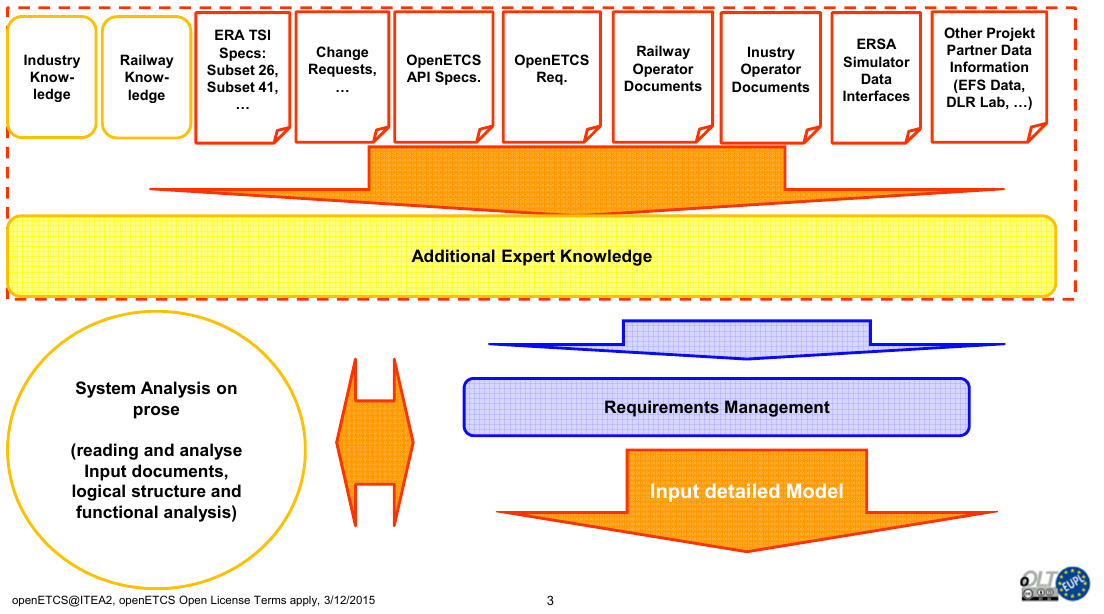
\includegraphics[scale=0.5]{images/AnalysisDocuments}
\caption{Analysis of input documents.}
\label{Analyising of input document}
\end{figure}

For a detailed discussion of the actual work process, please refer to the previous chapters. 

